\section{Evaluation}

\subsection{Implementation of Transfer Learning}

\subsection{Implementation of Siamese Network}

In this project, we implement both two loss functions with the architecture shown in figure \ref{fig:model}. Our network consists of a batch input layer and a deep CNN followed by L2 normalization, which results in the image embedding. This is followed by a loss function during training. Note that the siamese network was designed originally for the image matching task, not the image classification. Normally, it would have a distance function to compute the similarity between the two embedding vectors as the final outputs. However, our project is for the image classification problem, so we add one more CNN layer on top of that to train the embeddings to generate class output.

\begin{figure}[h]
  \centering
  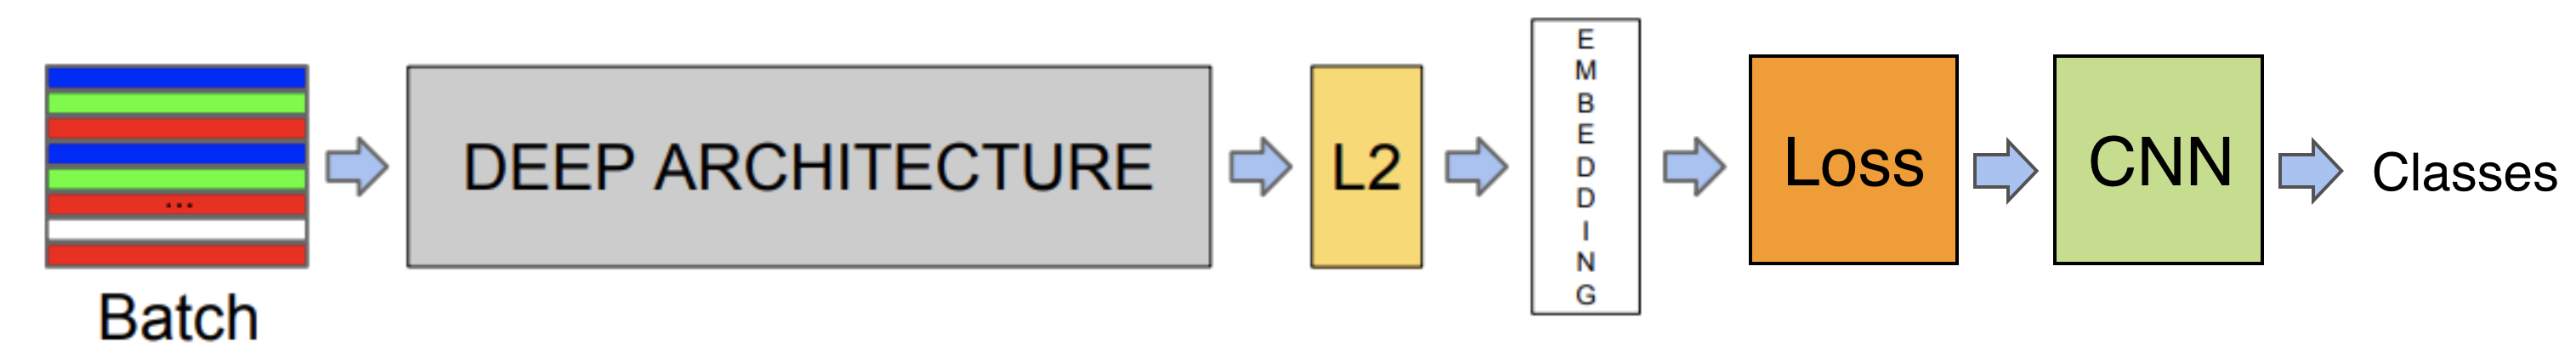
\includegraphics[width=\linewidth]{figs/model.png}
  \caption{The architecture of our model.}
  \label{fig:model}
\end{figure}

\subsubsection{Implementation of contrastive loss}
For contrastive loss, we implement and train siamese networks using Keras and Tensorflow. The implementation can be partitioned into three steps: 1) generating image pairs, 2) construct the architecture of the siamese neural network, 3) using contrastive loss to train the model. We adopt a simple strategy to make the image pairs. The positive sample is picked randomly from the same category as the anchor, and label with 1. On the other hand, we grab the negative sample randomly from classes that are different from the anchor and label it with 0. Figure \ref{fig:threesamples} shows the examples of the anchor, positive and negative samples. It's clear that the positive sample is much more similar to the anchor sample than the negative sample. Figure \ref{fig:contra_model} depicts the model we built. We can see all the hyperparameters from the figure. 

\begin{figure}[h]
  \centering
  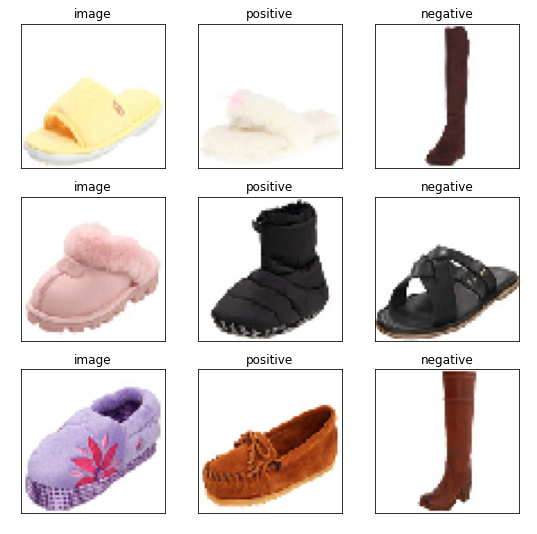
\includegraphics[width=0.9\linewidth]{figs/threesamples.png}
  \caption{Examples of anchor, positive and negative samples.}
  \label{fig:threesamples}
\end{figure}

\begin{figure}[h]
  \centering
  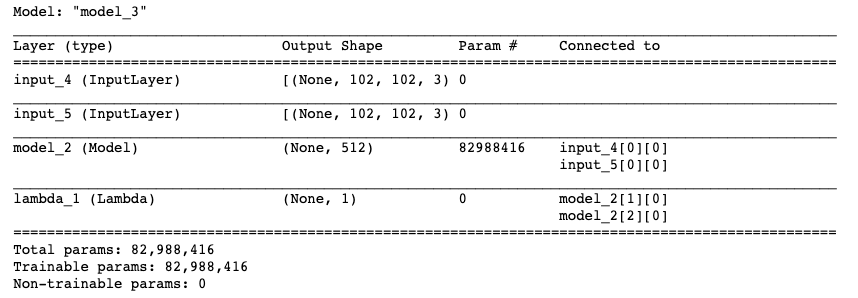
\includegraphics[width=\linewidth]{figs/contra_model.png}
  \caption{The model with contrastive loss we built.}
  \label{fig:contra_model}
\end{figure}

\subsubsection{Implementation of triplet loss}
We construct the model with triplet loss by calling the TripletSemiHardLoss function in TensorFlow Addons. As shown in the paper \cite{}, the best results are from Semi-Hard triplets. The negative is farther from the anchor than the positive, but still offers a positive loss. Figure \ref{fig:tri_model} illustrates the model. 

\begin{figure}[h]
  \centering
  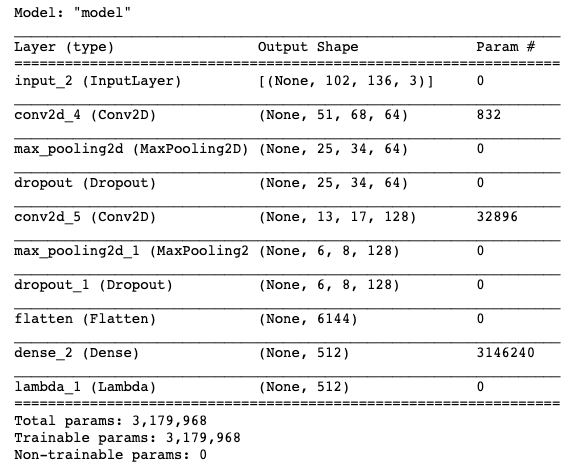
\includegraphics[width=\linewidth]{figs/tri_model.png}
  \caption{The model with triplet loss we built.}
  \label{fig:tri_model}
\end{figure}

\subsubsection{Combination of transfer Learning and triplet loss}
In this project, we also implement an advanced version that combine the transfer learning with triplet loss. We first use the Xception model to learn the embeddings of the three embeddings in a triplet. 



\subsection{Comparison and Analysis}

In this section, we first show the training loss for all the models, and we further analyze the effect of different hyperparameters. We then make a comparison of the results of all the models based on both the classification accuracy and the time-consume of training, and meanwhile, we give the possible reasons. Moreover, we not only focus on the overall classification accuracy but also the accuracy of each class. All our experiments are executed on the Cheaha with a single GPU. 

\subsubsection{Tranning Loss}

Figure \ref{fig:siatrainloss} shows the training loss for the three implementations of the siamese network. Figure \ref{ffig:tertrainloss} shows the training loss for the three implementations of the transfer Learning.


\begin{figure}[h]
  \centering
  \begin{subfigure}[b]{0.48\linewidth}
  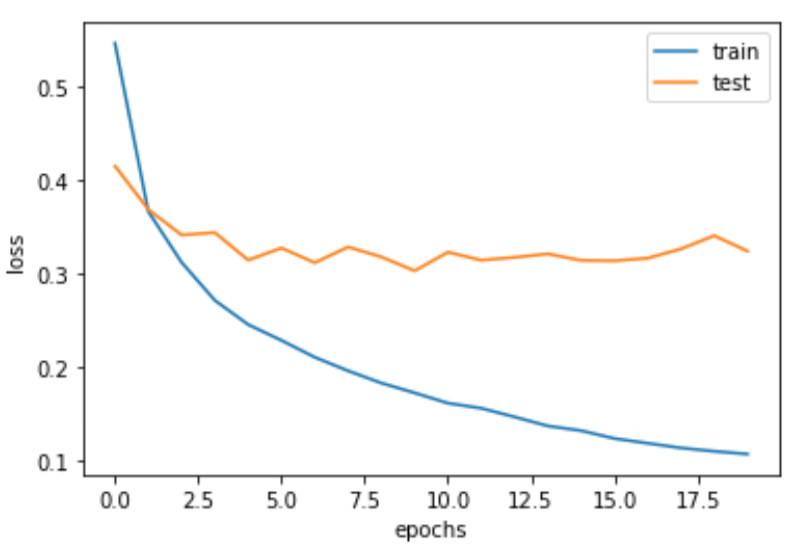
\includegraphics[width=\linewidth]{figs/transfer_loss.png}
  \caption{Transfer Learning version 1}
  \label{fig:con_loss}
  \end{subfigure}
  \hfill
   \begin{subfigure}[b]{0.48\linewidth}
   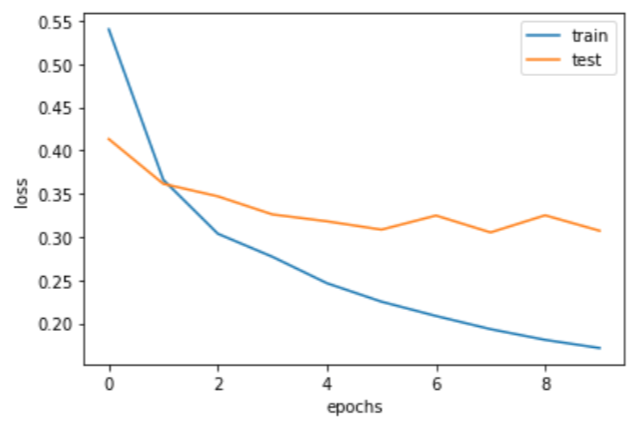
\includegraphics[width=\linewidth]{figs/transfer_loss_2.png}
   \caption{Transfer Learning version 2}
   \label{fig:tri_loss}
  \end{subfigure}
    \hfill
    \begin{subfigure}[b]{0.48\linewidth}
   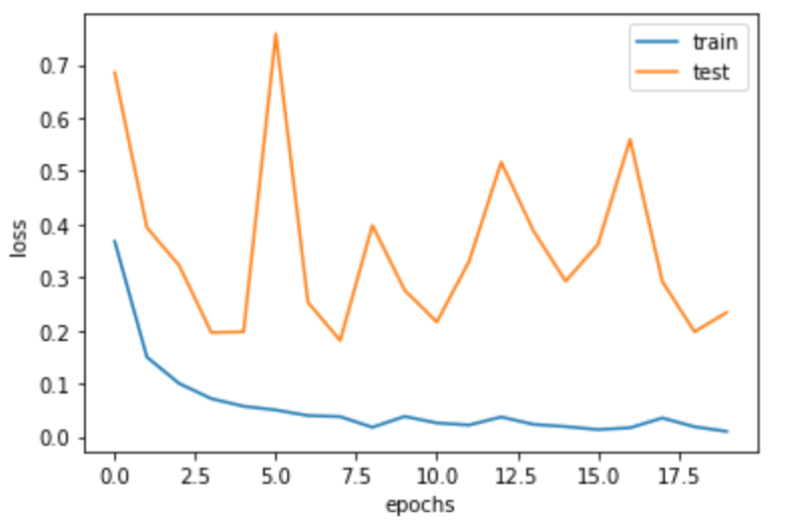
\includegraphics[width=\linewidth]{figs/transfer_loss_3.png}
   \caption{Transfer Learning version 3}
   \label{fig:tri_loss_2}
  \end{subfigure}
  \hfill
    \caption{Training loss of the three implementations of transfer Learning.}
    \label{fig:tertrainloss}
\end{figure}


\begin{figure}[h]
  \centering
  \begin{subfigure}[b]{0.48\linewidth}
  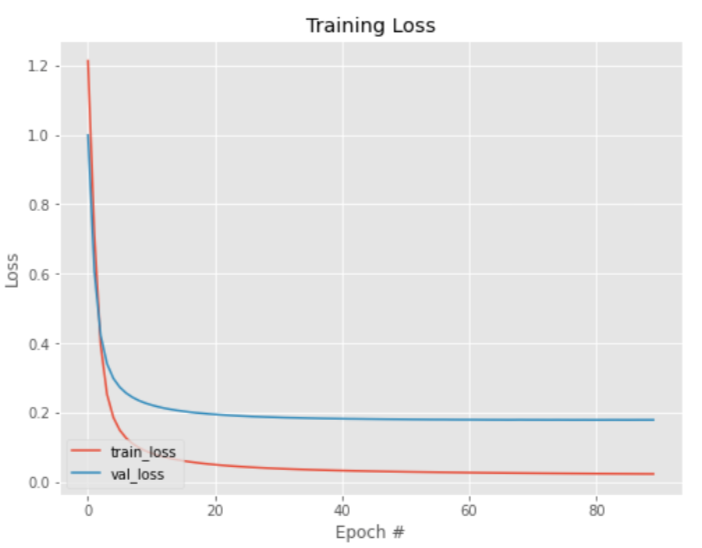
\includegraphics[width=\linewidth]{figs/con_loss.png}
  \caption{Contrastive loss}
  \label{fig:con_loss}
  \end{subfigure}
  \hfill
   \begin{subfigure}[b]{0.48\linewidth}
   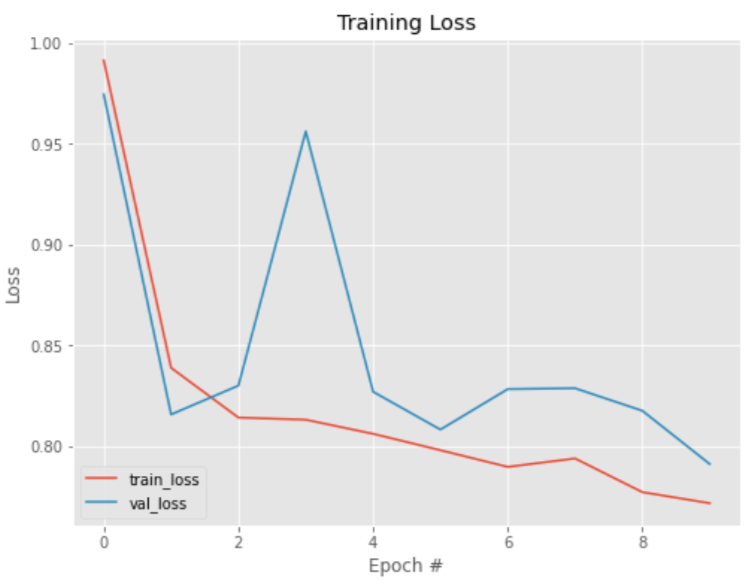
\includegraphics[width=\linewidth]{figs/tri_loss.png}
   \caption{Triplet loss}
   \label{fig:tri_loss}
  \end{subfigure}
    \hfill
    \begin{subfigure}[b]{0.48\linewidth}
   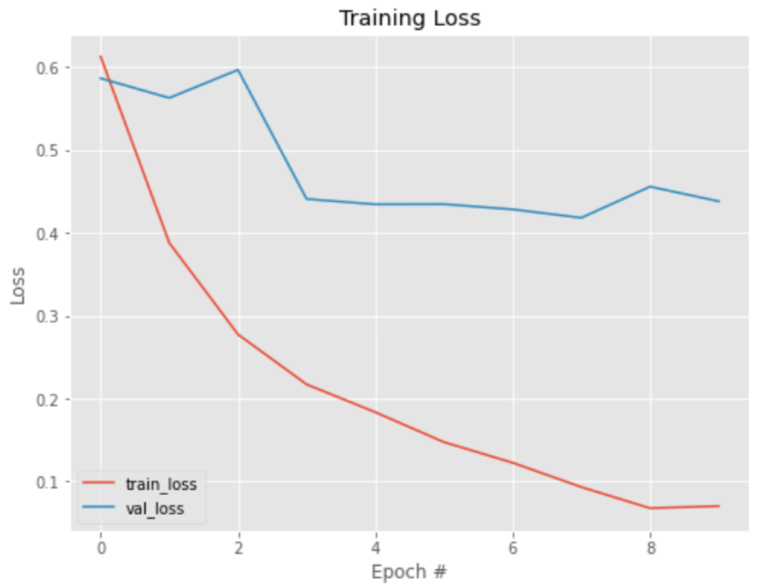
\includegraphics[width=\linewidth]{figs/tri_loss_2.png}
   \caption{Transfer Learning and triplet loss}
   \label{fig:tri_loss_2}
  \end{subfigure}
  \hfill
    \caption{Training loss of the three implementations of the siamese network.}
    \label{fig:siatrainloss}
\end{figure}

\subsubsection{Comparison}

\begin{figure}[h]
  \centering
  \begin{subfigure}[b]{0.48\linewidth}
  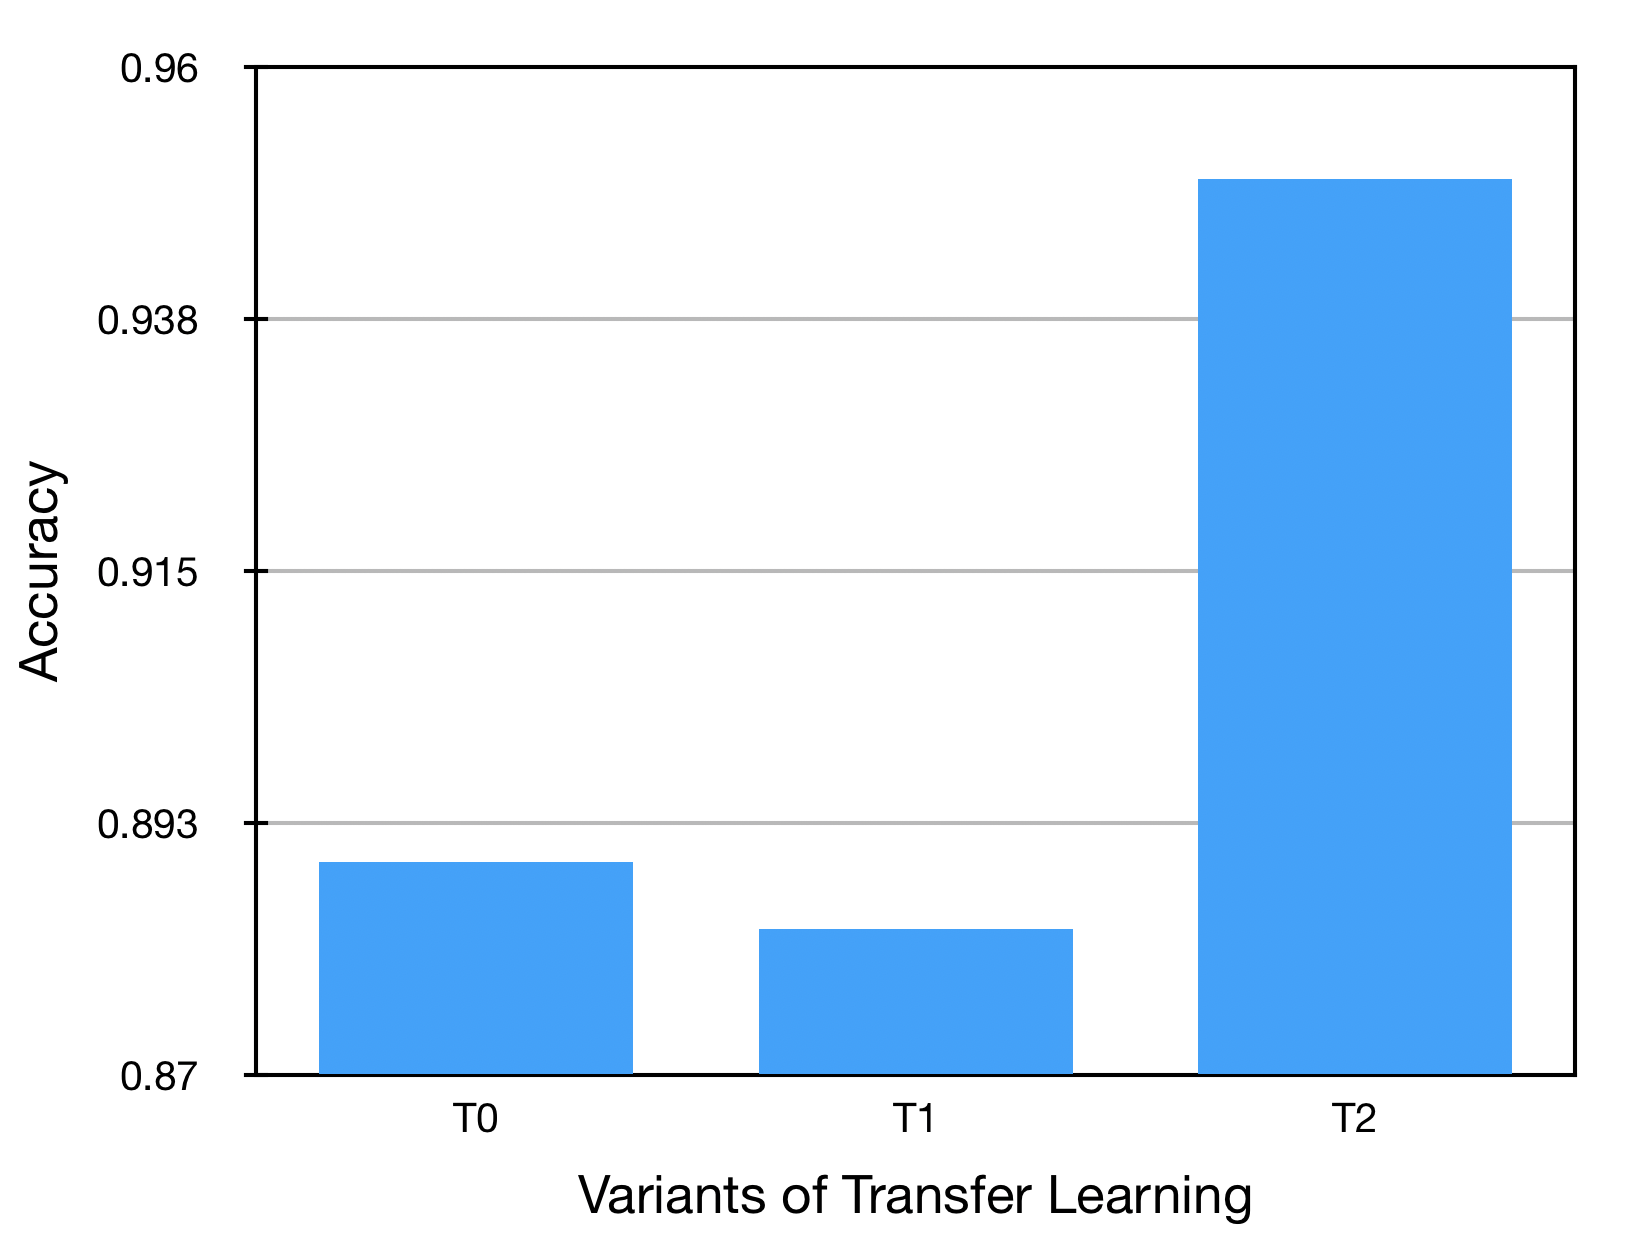
\includegraphics[width=\linewidth]{figs/acc_ter.png}
  \caption{Accuracy comparison}
  \label{fig:con_loss}
  \end{subfigure}
  \hfill
   \begin{subfigure}[b]{0.48\linewidth}
   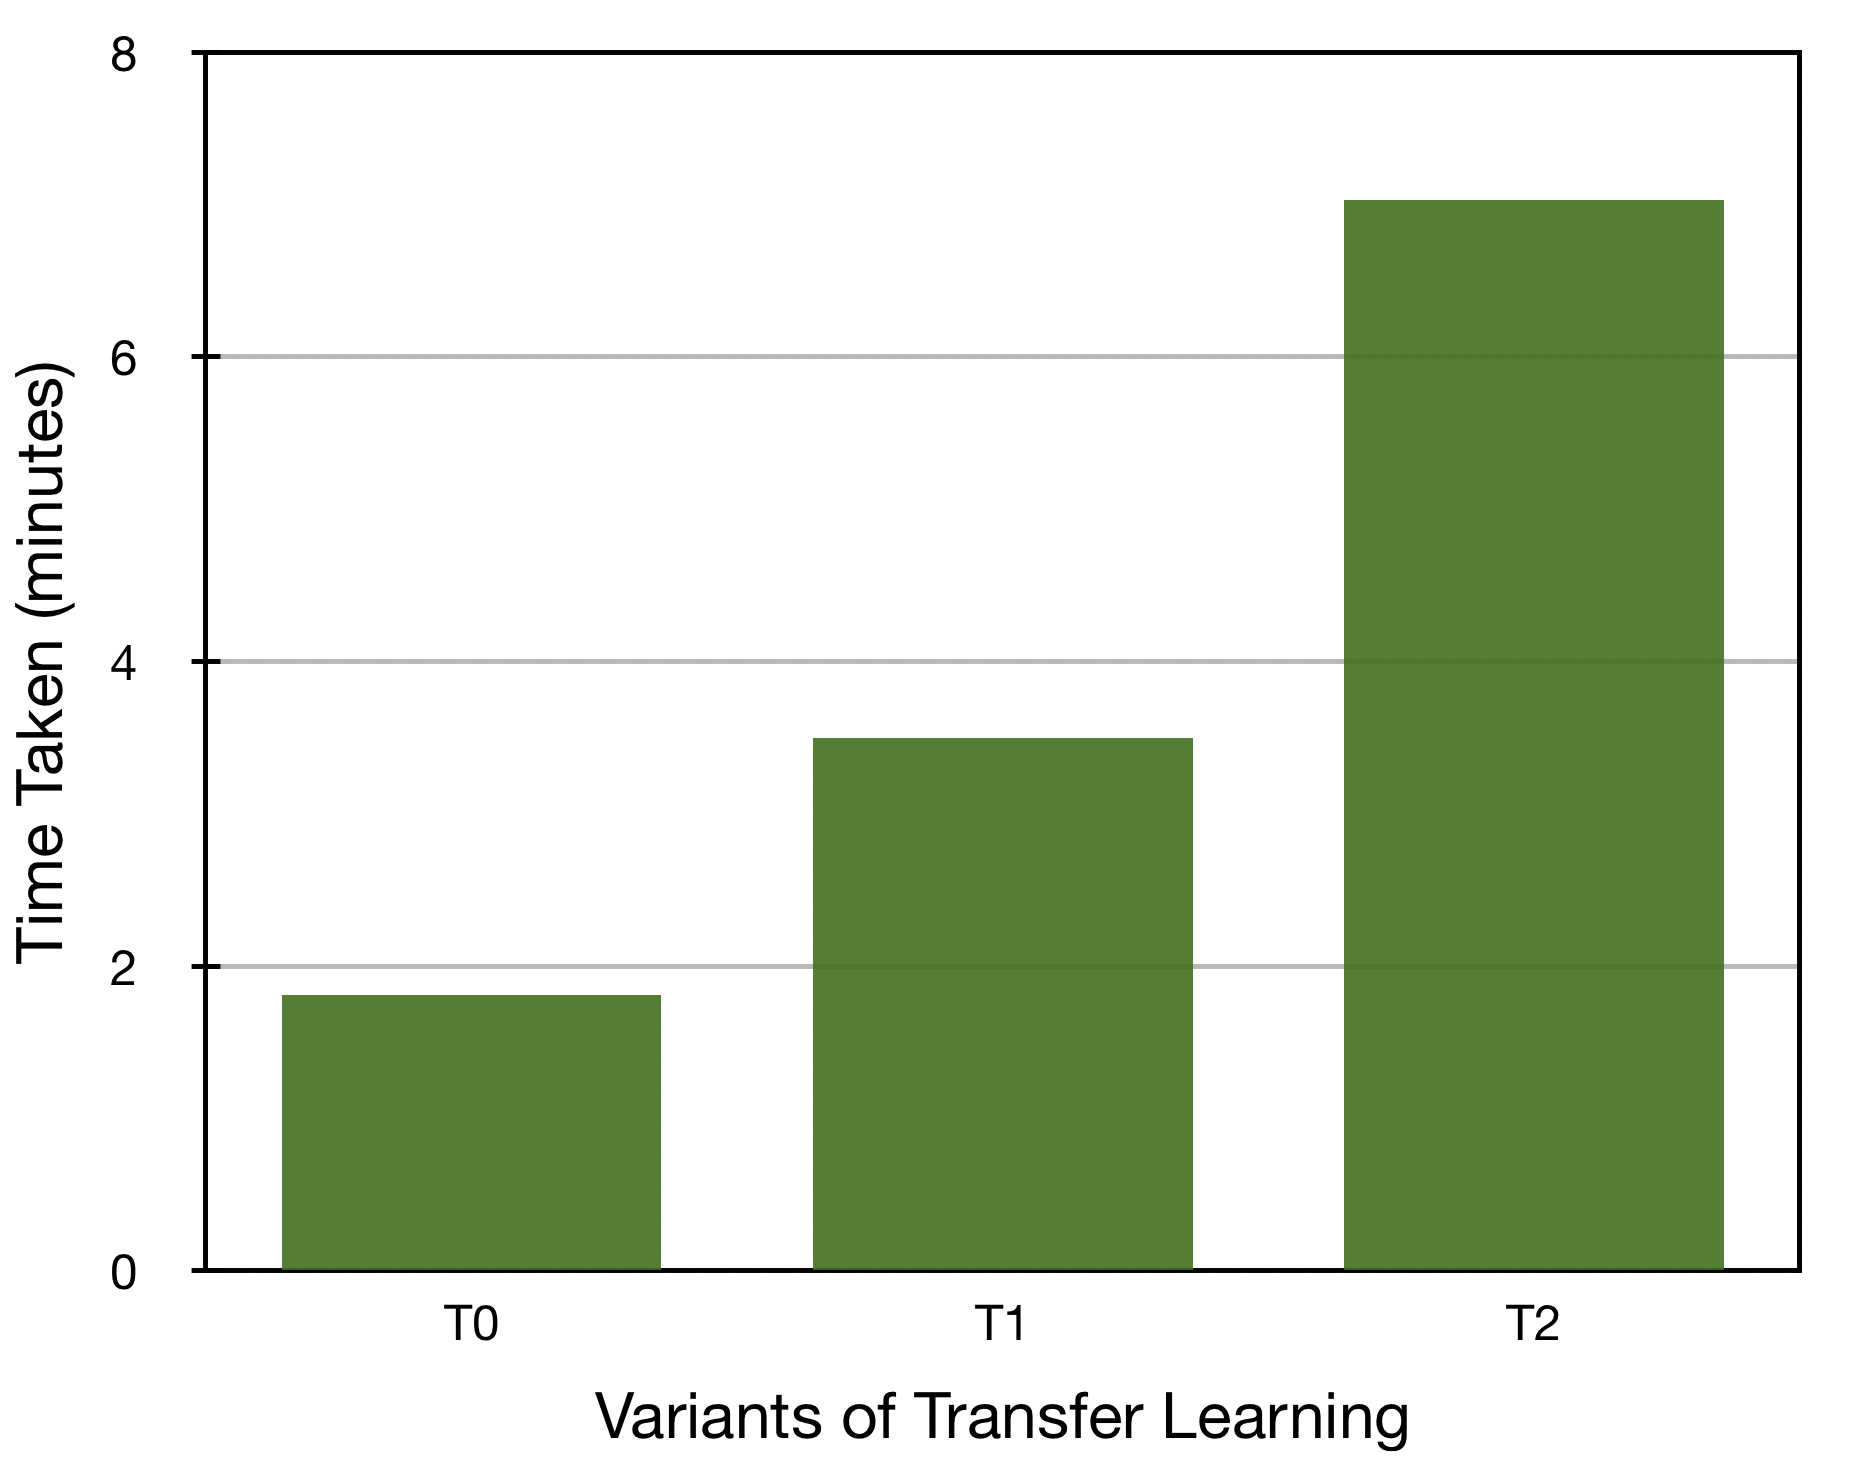
\includegraphics[width=\linewidth]{figs/time_ter.png}
   \caption{Time taken comparison}
   \label{fig:tri_loss}
  \end{subfigure}
    \hfill
    \caption{Comparison of the three implementations of the transfer learning.}
    \label{fig:siatrainloss}
\end{figure}

\begin{figure}[h]
  \centering
  \begin{subfigure}[b]{0.48\linewidth}
  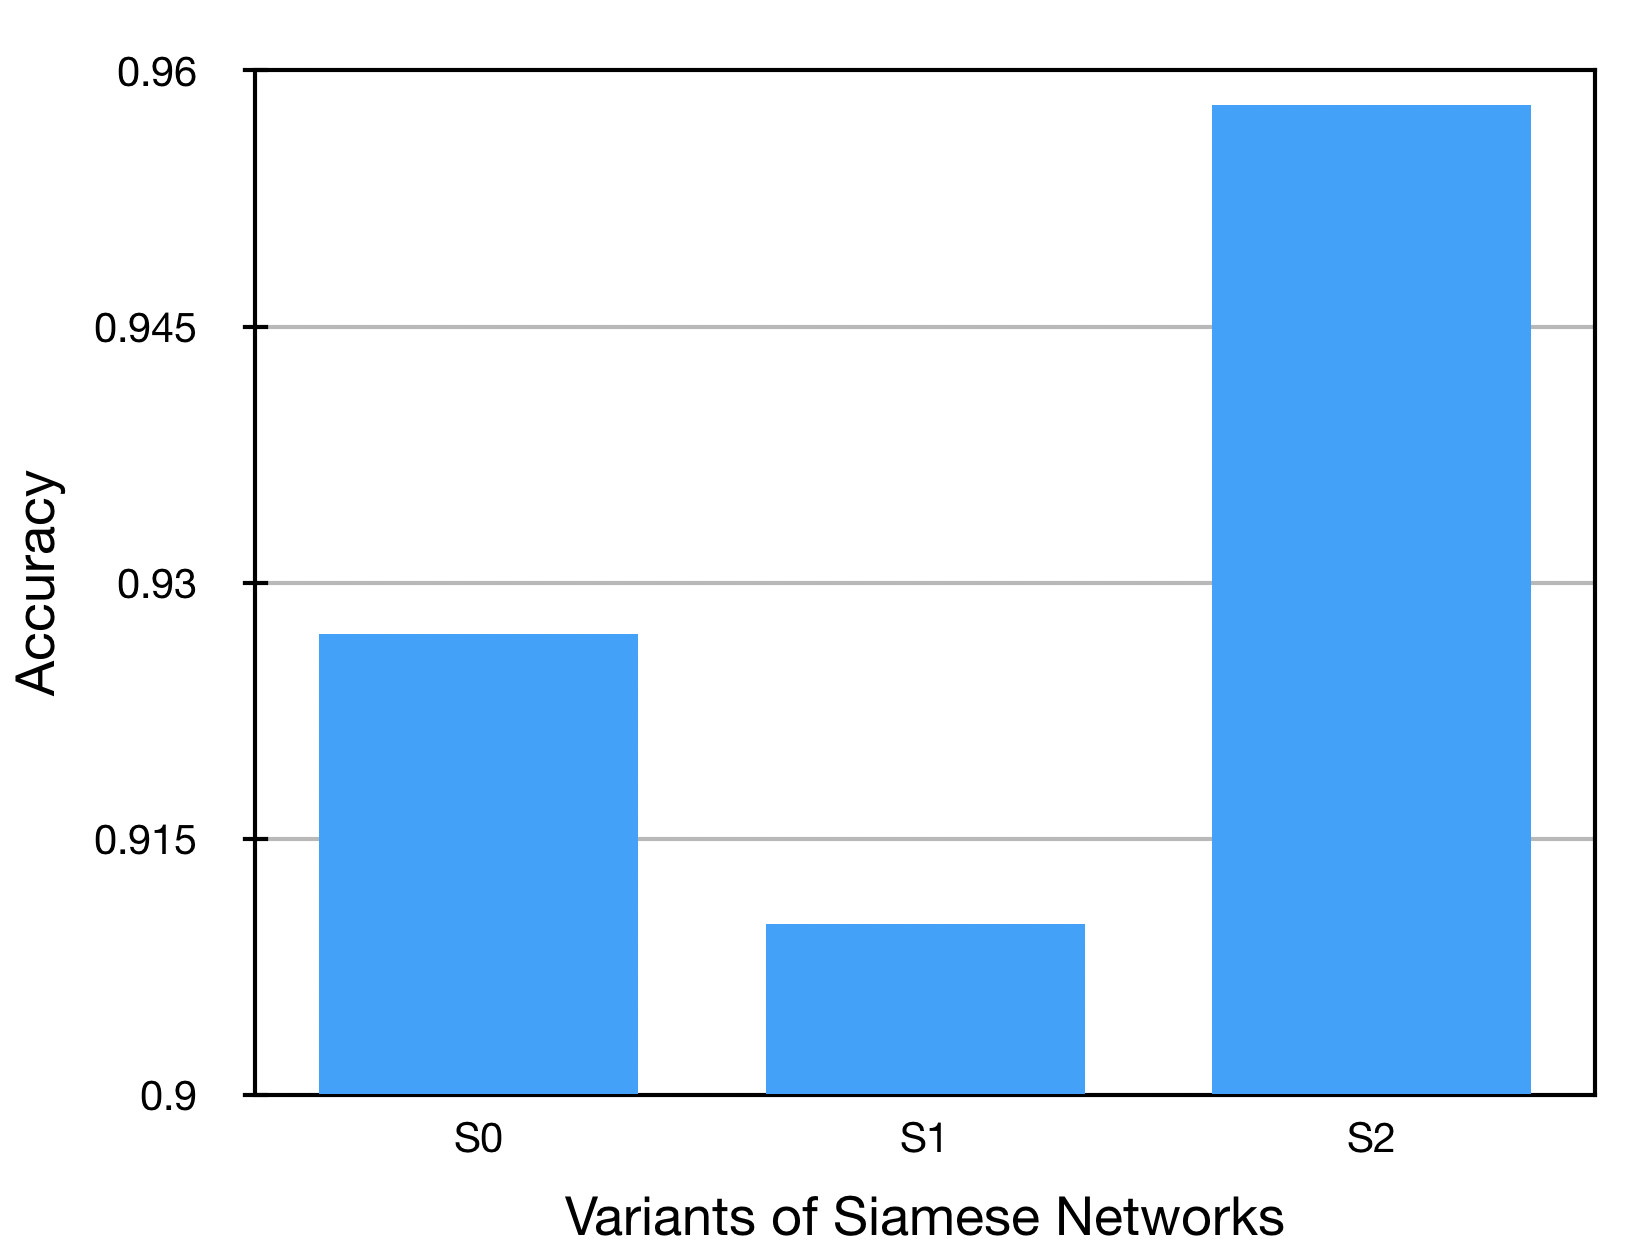
\includegraphics[width=\linewidth]{figs/acc_sia.png}
  \caption{Accuracy comparison}
  \label{fig:con_loss}
  \end{subfigure}
  \hfill
   \begin{subfigure}[b]{0.48\linewidth}
   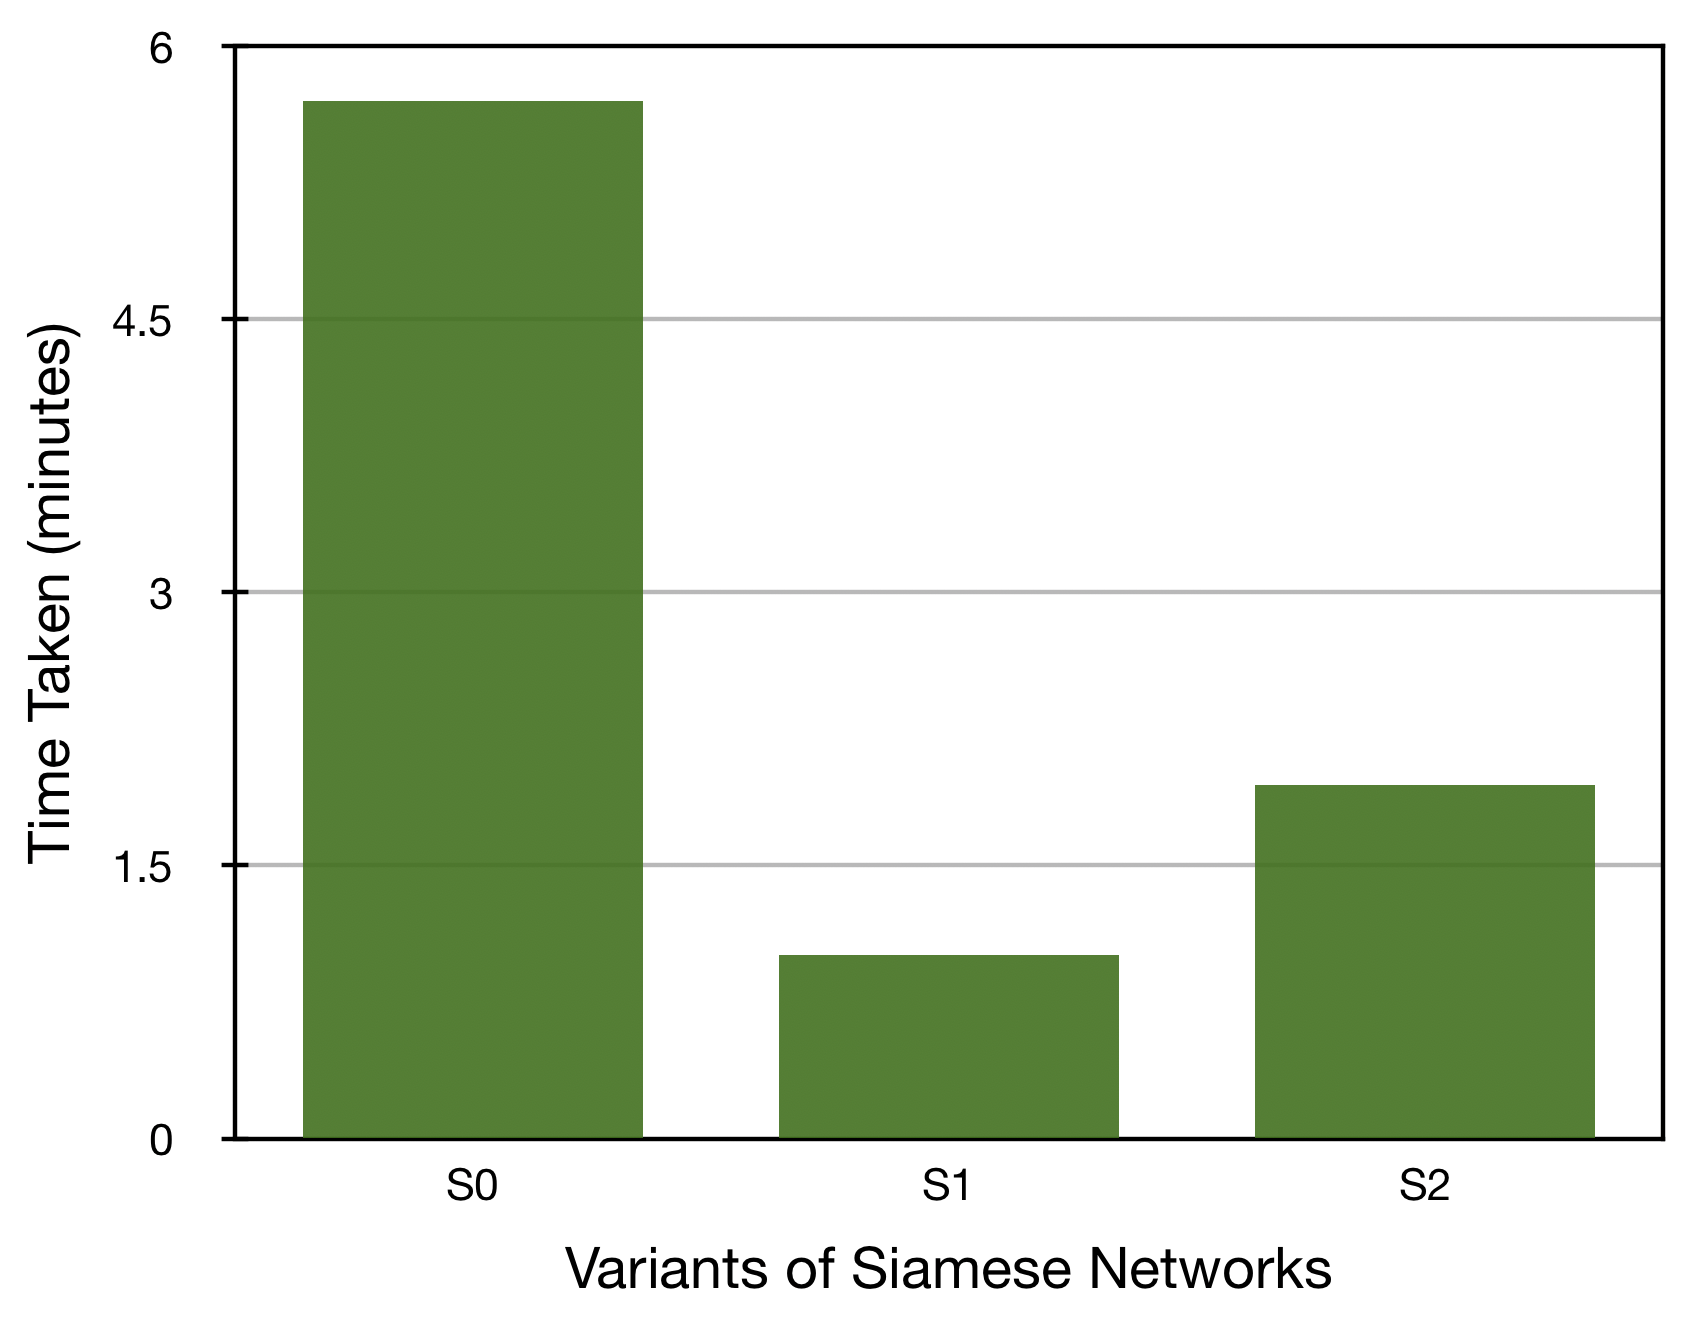
\includegraphics[width=\linewidth]{figs/time_sia.png}
   \caption{Time taken comparison}
   \label{fig:tri_loss}
  \end{subfigure}
    \hfill
    \caption{Comparison of the three implementations of the siamese network.}
    \label{fig:siatrainloss}
\end{figure}


\begin{figure}[h]
  \centering
  \begin{subfigure}[b]{0.48\linewidth}
  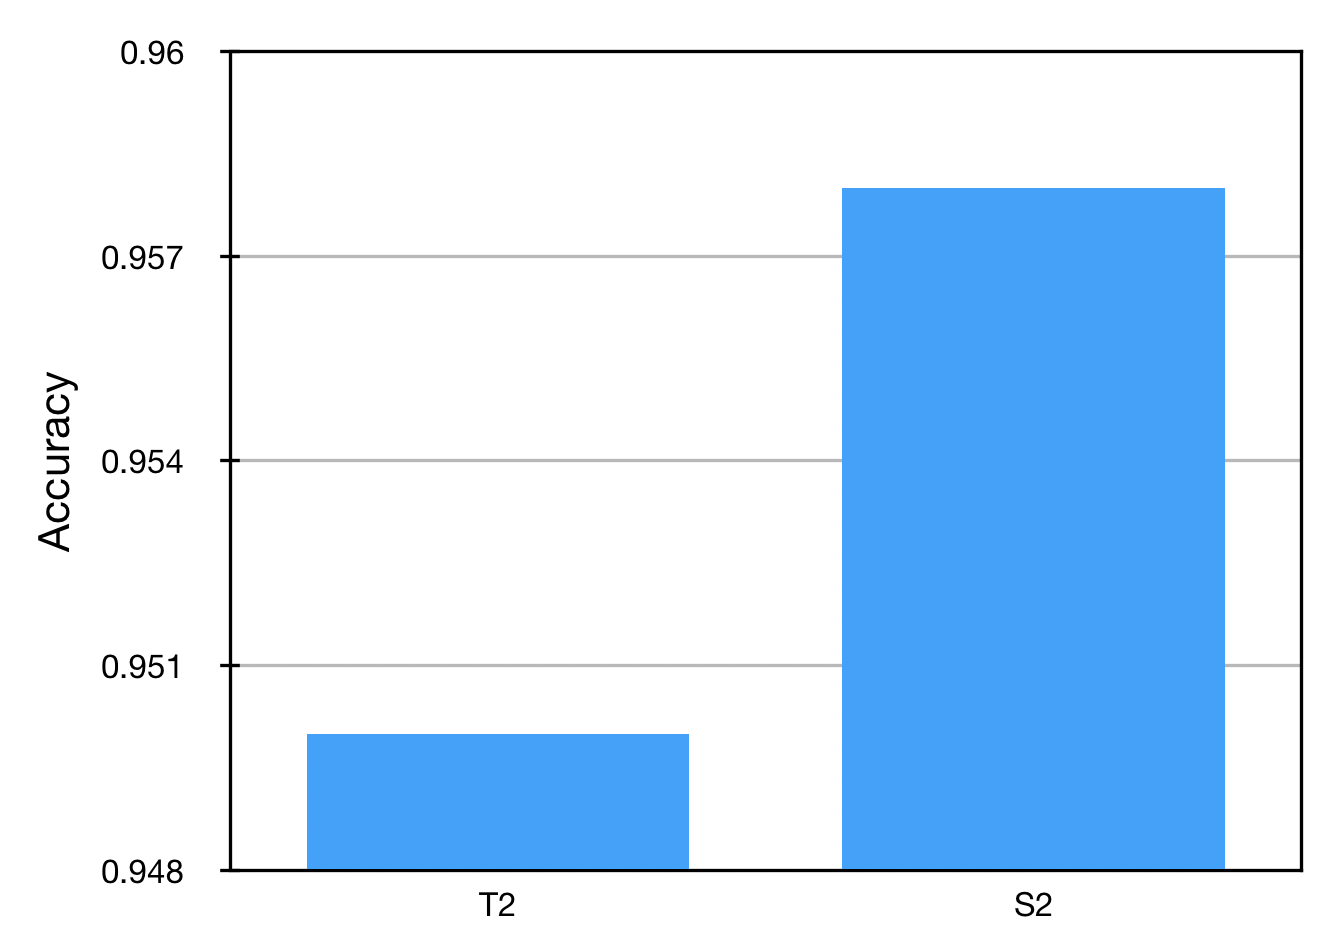
\includegraphics[width=\linewidth]{figs/acc.png}
  \caption{Accuracy comparison}
  \label{fig:con_loss}
  \end{subfigure}
  \hfill
   \begin{subfigure}[b]{0.48\linewidth}
   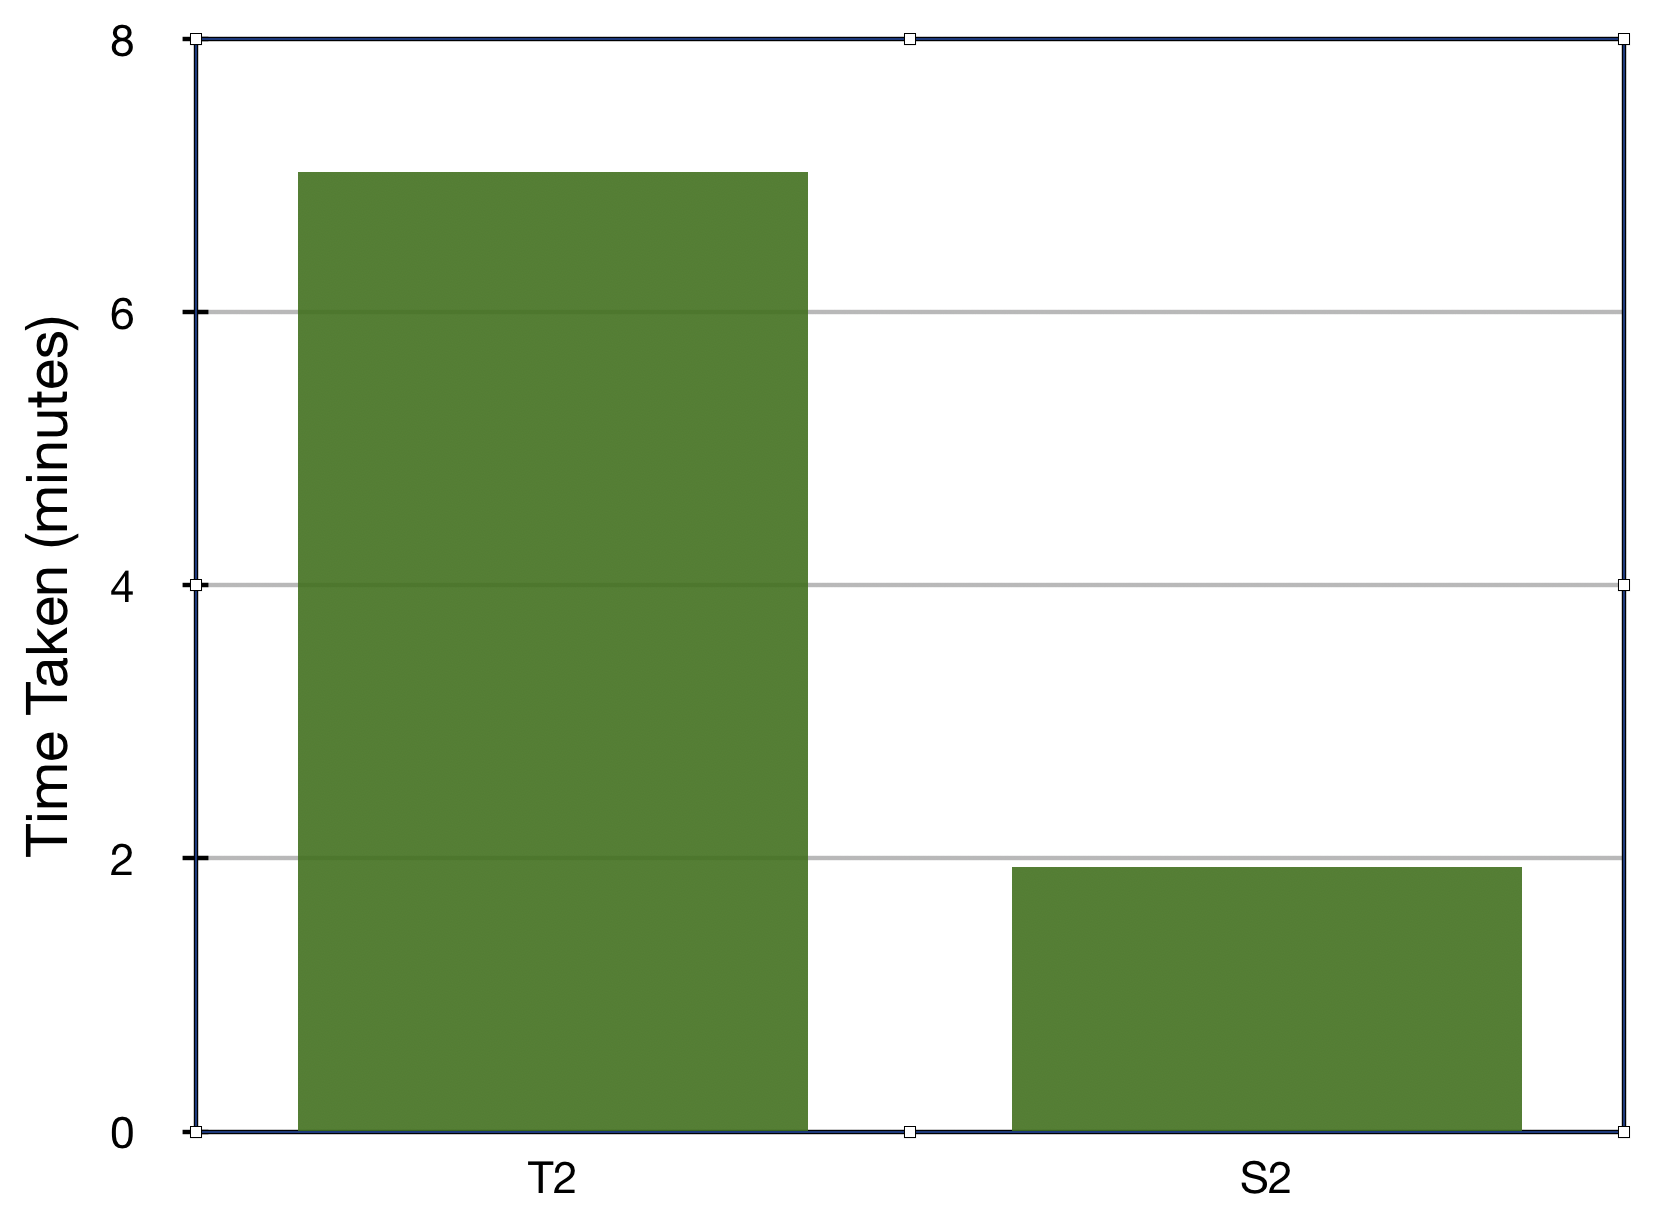
\includegraphics[width=\linewidth]{figs/time.png}
   \caption{Time taken comparison}
   \label{fig:tri_loss}
  \end{subfigure}
    \hfill
    \caption{Comparison of the two best implementaions.}
    \label{fig:siatrainloss}
\end{figure}




In our implementation, we observe that the triplet loss a little outperforms the contrastive loss. The possible reasons could be the triplet loss tries to be less greedy than contrastive loss since the distance is a relative concept. The triplet loss tries to bring the positive sample closer while also pushing away the negative sample when compared with an anchor, as shown in the figure \ref{fig:tripletloss}. In doing so, the model can clear know if the distance between the anchor sample and positive sample is smaller than the distance between the anchor and negative one. On the other hand, the contrastive loss, only considers one pair at a time, either positive or negative, so in a sense, it is more greedy. It's hard to ensure the similar objects are close enough. 

\begin{figure}[h]
  \centering
  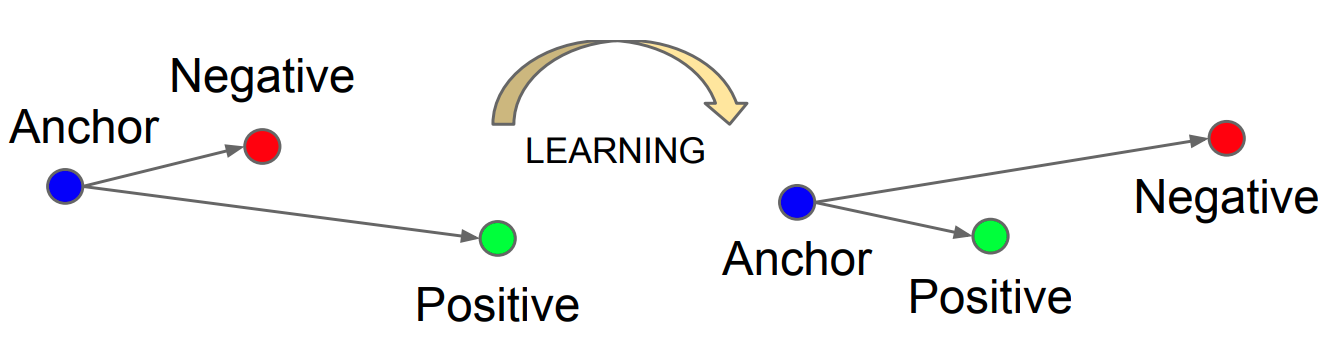
\includegraphics[width=\linewidth]{figs/tripletloss.png}
  \caption{The Triplet Loss minimizes the distance between an anchor and a positive, and maximizes the distance between the anchor and a negative.}
  \label{fig:tripletloss}
\end{figure}


Furthermore, we can also compute the similarity between image pairs, as shown in figure \ref{}. Note that the smaller distance between the two images means they are more similar to each other. For example, in the figure, the distance between the first pair is 0.12, and it turns out that they belong to the same class Slippers. As for the second pair, the class of left image is Slippers and the class of right image is Sandals. The distance between them is 0.56, which is much larger than the first pair, as we expected. 

\begin{figure}[h]
  \centering
  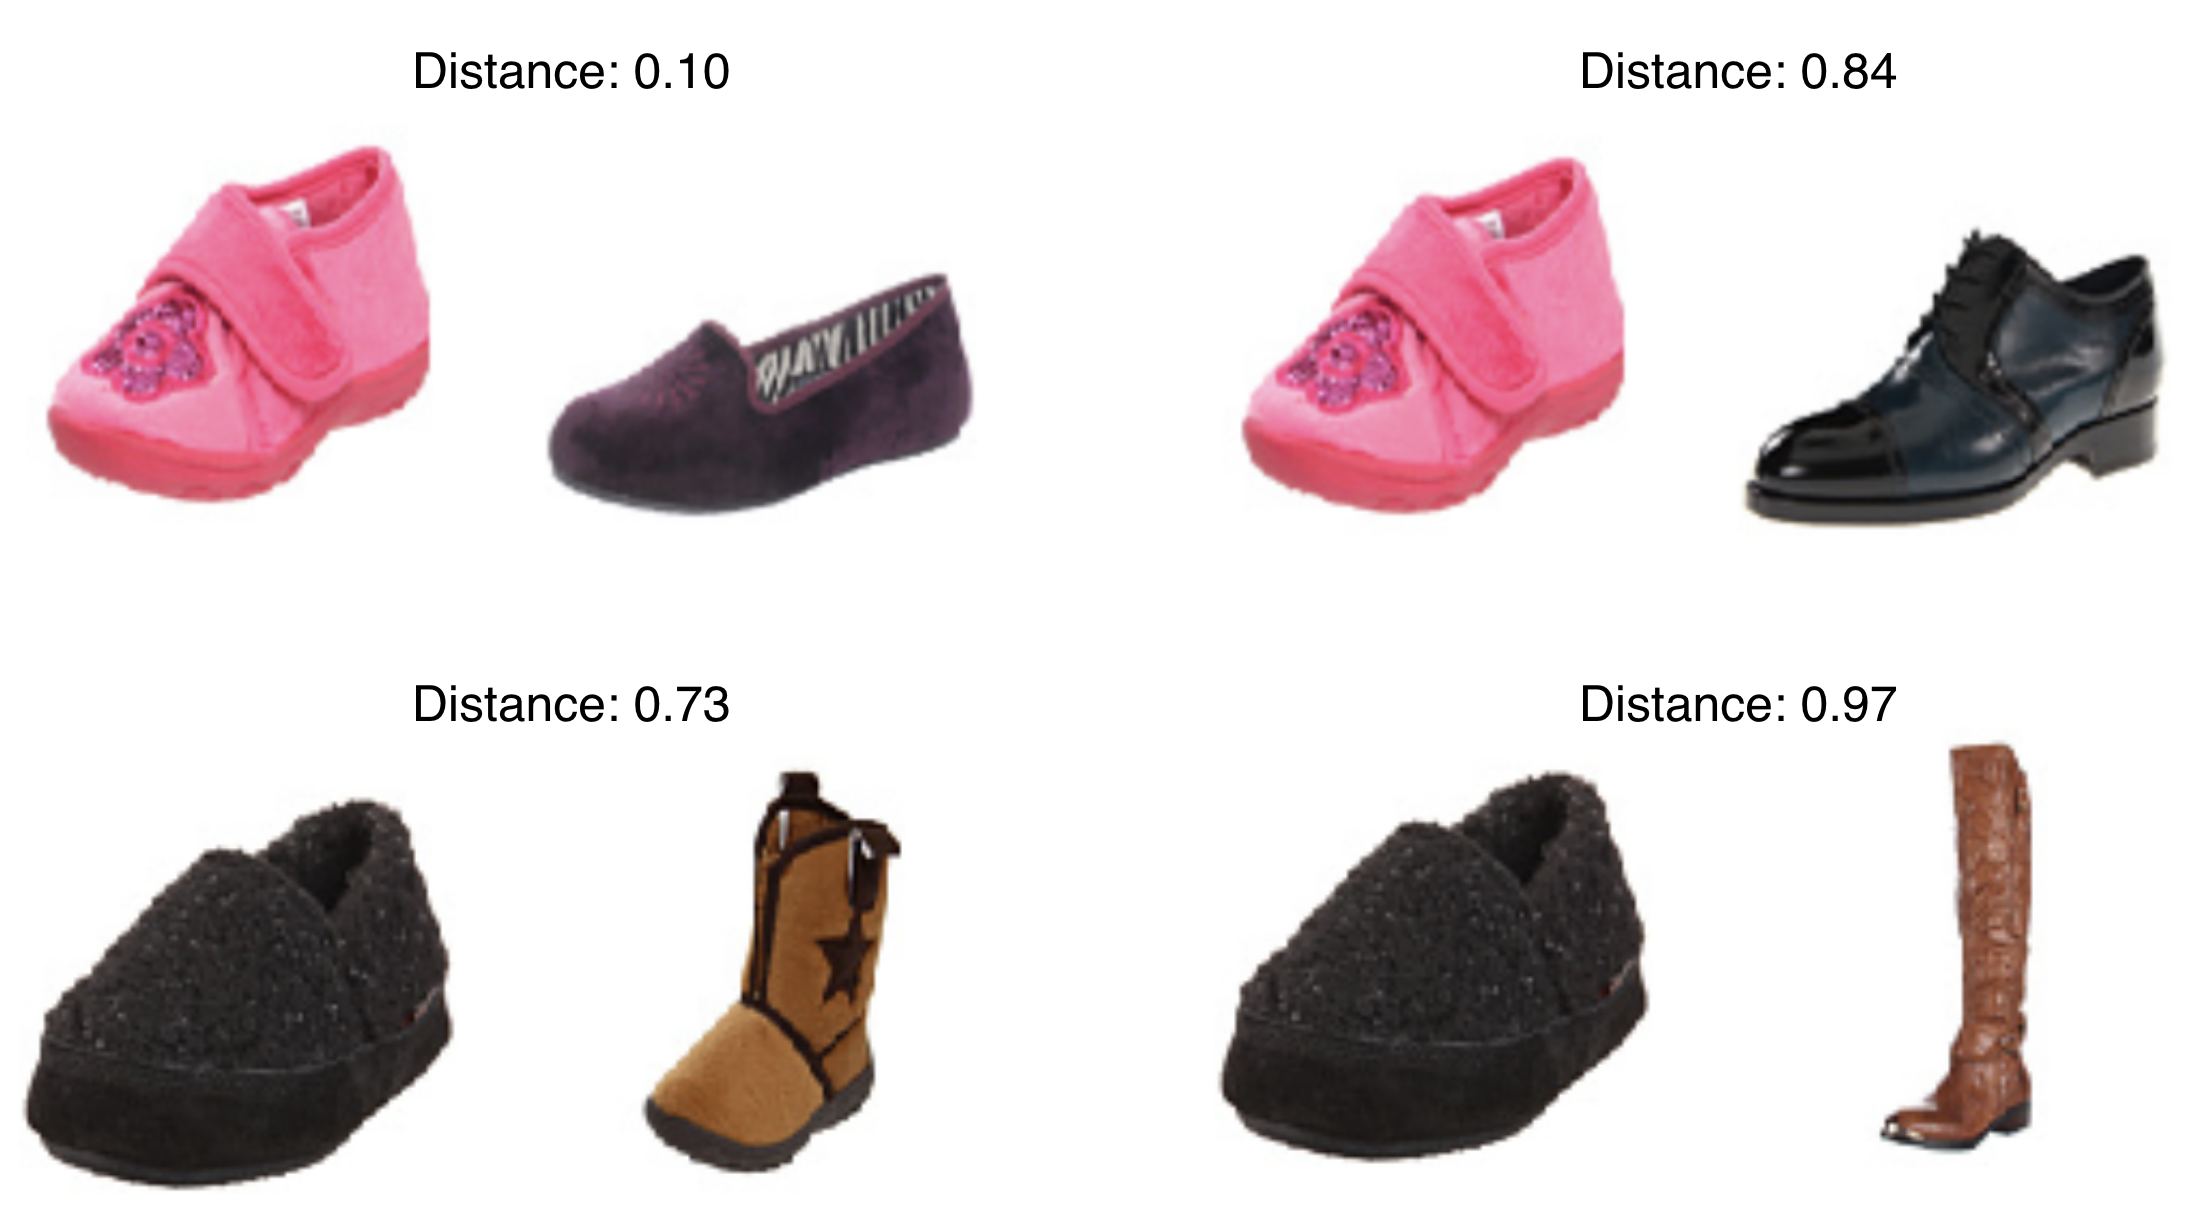
\includegraphics[width=\linewidth]{figs/similarity.png}
  \caption{Examples of calculating the similarity of image pairs.}
  \label{fig:similarity}
\end{figure}


